% Compile with pdflatex (twice for PDF links).
\documentclass[10pt,a4paper]{article}
\usepackage[margin=18mm]{geometry}
\usepackage[T1]{fontenc}
\usepackage{lmodern,amsmath,amssymb,booktabs,tabularx,array,xcolor,tikz}
\usepackage[colorlinks=true,urlcolor=teal,linkcolor=teal]{hyperref}
\hypersetup{pdftitle={Complex spatial rules: a practical decision note},pdfauthor={}}
\definecolor{ink}{HTML}{193747}
\definecolor{teal}{HTML}{087F8C}
\definecolor{pale}{HTML}{EDF6F6}
\definecolor{amber}{HTML}{A36016}
\definecolor{muted}{HTML}{52636D}
\setlength{\parindent}{0pt}
\setlength{\parskip}{5pt}
\renewcommand{\arraystretch}{1.18}
\newcolumntype{Y}{>{\raggedright\arraybackslash}X}
\newcommand{\heading}[1]{\par\vspace{5pt}{\large\bfseries\color{ink}#1}\par\vspace{2pt}}
\newcommand{\eyebrow}[1]{{\small\sffamily\bfseries\color{teal}#1}\par}
\newcommand{\note}[1]{\par\noindent\colorbox{pale}{\parbox{\dimexpr\linewidth-2\fboxsep\relax}{#1}}\par}
\newcommand{\smalltext}[1]{{\small\color{muted}#1}\par}
\newcommand{\A}{A}
\begin{document}
\color{ink}
\eyebrow{DECISION NOTE\quad /\quad BINARY PATCH PRESENCE}
{\LARGE\bfseries Complex spatial rules}\par
{\large What to keep, what to compare, and what the tests establish}

\note{\textbf{Recommendation.} Keep lift and your $I$. For $A,B\to C$, also check the gain over $B\to C$ and test that second gain. A large $I$ alone can be entirely explained by $B\to C$.}

\heading{1\quad One population, two contributions}
$A$ means \textbf{center type A}; $B,C$ mean \textbf{distinct neighbor types present}. Count each retained patch once, within one sample. All unconditioned counts use the same patches across \emph{all} center types. Write $n_{ABC}$ for patches containing all three events, and similarly for other counts.

\begin{center}
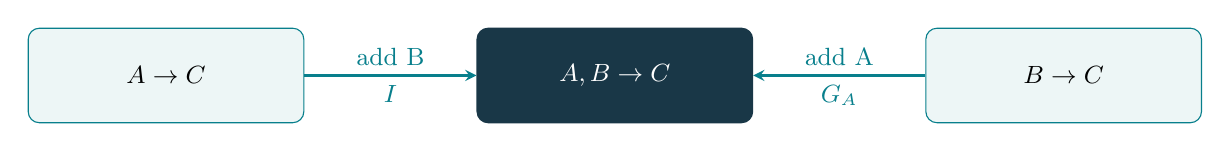
\begin{tikzpicture}[every node/.style={font=\small},>=stealth]
\node[draw=teal,fill=pale,rounded corners,minimum width=35mm,minimum height=12mm] (left) at (0,0) {$A\to C$};
\node[draw=ink,fill=ink,text=white,rounded corners,minimum width=35mm,minimum height=12mm] (middle) at (5.7,0) {$A,B\to C$};
\node[draw=teal,fill=pale,rounded corners,minimum width=35mm,minimum height=12mm] (right) at (11.4,0) {$B\to C$};
\draw[->,thick,teal] (left) -- node[above]{add B} node[below]{$I$} (middle);
\draw[->,thick,teal] (right) -- node[above]{add A} node[below]{$G_A$} (middle);
\end{tikzpicture}
\end{center}
\vspace{-3mm}
\begin{align*}
 I&=\frac{P(C\mid AB)}{P(C\mid A)}
   =\frac{P(BC\mid A)}{P(B\mid A)P(C\mid A)}
   =\frac{n_{ABC}n_A}{n_{AB}n_{AC}},\\
 G_A&=\frac{P(C\mid AB)}{P(C\mid B)}
   =\frac{n_{ABC}n_B}{n_{AB}n_{BC}}.
\end{align*}
\textbf{$I$ asks whether B adds information beyond A; $G_A$ asks whether A adds information beyond B.} A gain of 1.2 is a 20\% relative increase, not 20 percentage points. $I$ is symmetric in B and C; the prediction rule and $G_A$ are directional.

\begin{center}
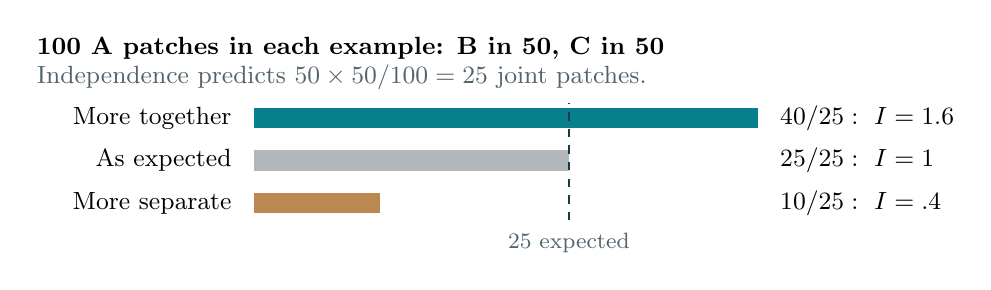
\begin{tikzpicture}[x=.16cm,y=.54cm,every node/.style={font=\small}]
\node[anchor=west,font=\small\bfseries] at (-18,3.65) {100 A patches in each example: B in 50, C in 50};
\node[anchor=west,text=muted] at (-18,2.95) {Independence predicts $50\times50/100=25$ joint patches.};
\fill[amber!75] (0,-.24) rectangle (10,.24);
\fill[muted!45] (0,.76) rectangle (25,1.24);
\fill[teal] (0,1.76) rectangle (40,2.24);
\draw[dashed,ink,thick] (25,-.4) -- (25,2.35);
\node[anchor=east] at (-1,2) {More together};
\node[anchor=east] at (-1,1) {As expected};
\node[anchor=east] at (-1,0) {More separate};
\node[anchor=west] at (41,2) {$40/25:\ I=1.6$};
\node[anchor=west] at (41,1) {$25/25:\ I=1$};
\node[anchor=west] at (41,0) {$10/25:\ I=.4$};
\node[anchor=north,text=muted,font=\footnotesize] at (25,-.48) {25 expected};
\end{tikzpicture}
\end{center}
\vspace{-3mm}

\heading{2\quad Recommended gates}
The two rule lifts use different baselines:
\[
 L_J=\frac{P(BC\mid A)}{P(BC)},\qquad
 L_K=\frac{P(C\mid AB)}{P(C)}.
\]
\begin{tabularx}{\linewidth}{@{}p{23mm}YY@{}}
\toprule
\textbf{Positive rule}&\textbf{Effect criteria}&\textbf{Meaning in the observed data}\\
\midrule
$A\to B,C$ & $L_J\ge1.2$, $I\ge1.2$ & BC is enriched around A and exceeds the product of its two frequencies within A.\\
$A,B\to C$ & $L_K\ge1.2$, $I\ge1.2$, $G_A\ge1.2$ & C is enriched and prediction improves over either antecedent alone.\\
\bottomrule
\end{tabularx}

\textbf{Significance:} retain the rule's own permutation $q_{\rm rule}\le.05$. Also require $q_I\le.05$ for $A\to B,C$, or the combined $q_{\rm add}\le.05$ for $A,B\to C$ (page 2).

\textbf{Negative rules:} replace each effect threshold by $\le1/1.2\approx.833$; retain the significance gates. Complex antecedents must improve avoidance over \emph{both} simpler predictions. A negative joint rule describes fewer BC combinations, not necessarily avoidance of each neighbor individually.

\note{\textbf{Keep roles explicit.} Here $B\to C$ means B-neighbor presence predicting C-neighbor presence in the original patches. Your code's B-center$\to$C-neighbor comparator changes the patch geometry. It answers a different biological question.}

\smalltext{These criteria support the descriptive claims above. They do not establish causation or a B--C interaction stronger around A than elsewhere. Spatial calibration governs the statistical confidence, not the arithmetic.}

\newpage
\eyebrow{CALCULATION\quad /\quad TWO TABLES, THEN ONE RULE-LEVEL CORRECTION}
\heading{3\quad Apply the same Fisher test twice}
\begin{minipage}[t]{.48\linewidth}
\textbf{B adds beyond A}\par
Restrict to A-centered patches.\par
\centering
\small
\begin{tabular}{@{}lcc@{}}
\toprule
 & C & No C\\\midrule
B & $n_{ABC}$ & $n_{AB}-n_{ABC}$\\
No B & $n_{AC}-n_{ABC}$ & $\substack{n_A-n_{AB}\\-n_{AC}+n_{ABC}}$\\
\bottomrule
\end{tabular}\par
\raggedright $p_B$: Fisher test of $I=1$.
\end{minipage}\hfill
\begin{minipage}[t]{.48\linewidth}
\textbf{A adds beyond B}\par
Restrict to B-containing patches.\par
\centering
\small
\begin{tabular}{@{}lcc@{}}
\toprule
 & C & No C\\\midrule
A & $n_{ABC}$ & $n_{AB}-n_{ABC}$\\
Not A & $n_{BC}-n_{ABC}$ & $\substack{n_B-n_{AB}\\-n_{BC}+n_{ABC}}$\\
\bottomrule
\end{tabular}\par
\raggedright $p_A$: Fisher test of $G_A=1$.
\end{minipage}

Use two-sided Fisher tests, then require the desired effect direction. Fisher tests odds ratio 1; the odds ratio itself is \emph{not} $I$ or $G_A$. For any table $\left[\begin{smallmatrix}a&b\\c&d\end{smallmatrix}\right]$, with $N=a+b+c+d$ and fixed margins:
\[
 h(x)=\frac{\binom{a+c}{x}\binom{b+d}{a+b-x}}{\binom{N}{a+b}},
 \qquad p=\sum_{x:\,h(x)\le h(a)}h(x).
\]
\textbf{For complex antecedents, the weaker comparison decides:}
\begin{center}
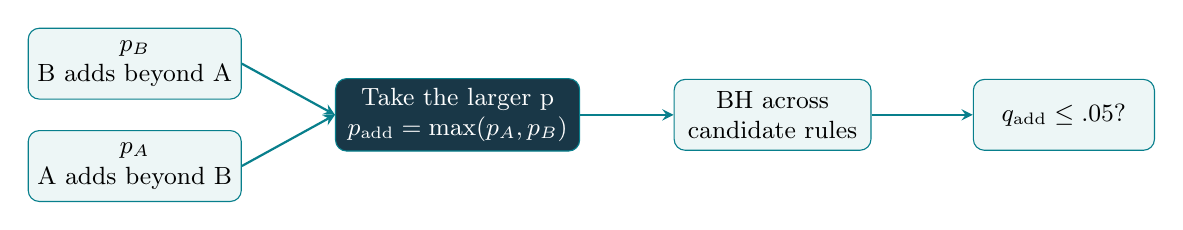
\begin{tikzpicture}[every node/.style={font=\small},>=stealth,
 box/.style={draw=teal,fill=pale,rounded corners,align=center,minimum height=9mm}]
\node[box,minimum width=23mm] (pb) at (0,.65) {$p_B$\\B adds beyond A};
\node[box,minimum width=23mm] (pa) at (0,-.65) {$p_A$\\A adds beyond B};
\node[box,fill=ink,text=white,minimum width=31mm] (max) at (4.1,0) {Take the larger p\\$p_{\rm add}=\max(p_A,p_B)$};
\node[box,minimum width=25mm] (bh) at (8.1,0) {BH across\\candidate rules};
\node[box,minimum width=23mm] (q) at (11.8,0) {$q_{\rm add}\le.05$?};
\draw[->,thick,teal] (pb.east) -- (max.west);
\draw[->,thick,teal] (pa.east) -- (max.west);
\draw[->,thick,teal] (max) -- (bh);
\draw[->,thick,teal] (bh) -- (q);
\end{tikzpicture}
\end{center}
\vspace{-2mm}
BH sorts the $m$ raw combined p-values and uses
$q_{(i)}=\min\{1,\min_{j\ge i}m p_{(j)}/j\}$.
Both comparisons must succeed. If either independence null is true, a small maximum requires its p-value to be small too. This combination is valid when its component tests are valid, even if they depend on each other.

Apply BH to all planned complex-antecedent candidates per sample, including attraction and avoidance, before selecting favorable results. For joint rules, correct $p_B$ separately across centered triplets with unordered \{B,C\}, giving $q_I$. Missing comparators must be measured from the patches; missing or untestable values cannot pass.

\heading{4\quad The pitfall and a rule that survives it}
\textbf{How often is C present?} Both panels use the same 0--100\% scale.
\begin{center}
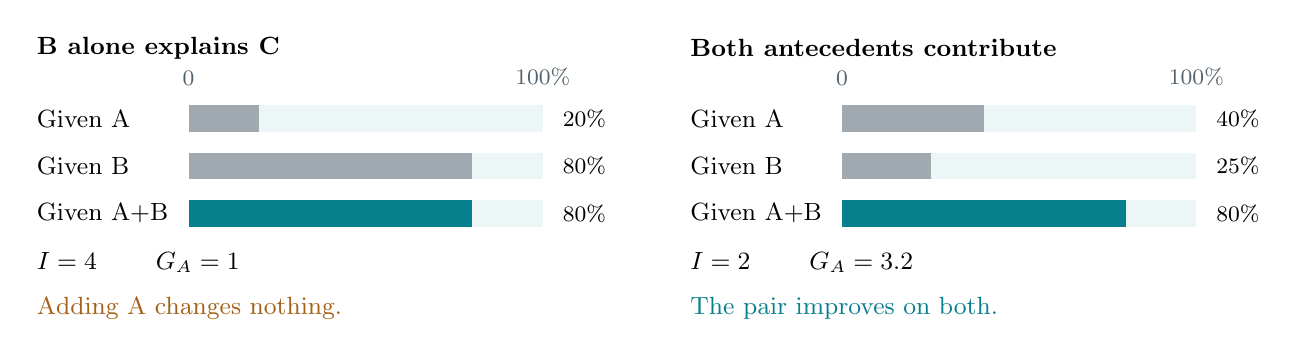
\begin{tikzpicture}[x=1cm,y=1cm,every node/.style={font=\small}]
\foreach \shift/\title/\aval/\bval/\igain/\again in {0/{B alone explains C}/20/80/4/1,8.3/{Both antecedents contribute}/40/25/2/3.2}{
\begin{scope}[xshift=\shift cm]
\node[anchor=west,font=\small\bfseries] at (0,2.1) {\title};
\foreach \row/\label/\val/\shade in {1.2/{Given A}/\aval/{muted!55},.6/{Given B}/\bval/{muted!55},0/{Given A+B}/80/{teal}}{
\node[anchor=west] at (0,\row) {\label};
\fill[pale] (2.05,\row-.17) rectangle (6.55,\row+.17);
\fill[\shade] (2.05,\row-.17) rectangle ({2.05+.045*\val},\row+.17);
\node[anchor=west,font=\footnotesize] at (6.68,\row) {\val\%};
}
\node[anchor=south,text=muted,font=\footnotesize] at (2.05,1.5) {0};
\node[anchor=south,text=muted,font=\footnotesize] at (6.55,1.5) {100\%};
\node[anchor=west,font=\small\bfseries] at (0,-.62) {$I=\igain\qquad G_A=\again$};
\end{scope}
}
\node[anchor=west,text=amber] at (0,-1.2) {Adding A changes nothing.};
\node[anchor=west,text=teal] at (8.3,-1.2) {The pair improves on both.};
\end{tikzpicture}
\end{center}
\vspace{-2mm}
Both examples have 100 A patches among 1,000 total patches. Counts are $(n_{AB},n_{AC},n_{ABC});(n_B,n_C,n_{BC})$; both have $L_K=4$.

\begin{tabularx}{\linewidth}{@{}p{29mm}YY@{}}
\toprule
&\textbf{B alone explains C}&\textbf{Both antecedents contribute}\\\midrule
Counts & $(20,20,16);(200,200,160)$ & $(20,40,16);(200,200,50)$\\
Fisher $p_B,\ p_A$ & $1.45\!\times\!10^{-11},\ 1$ & $7.11\!\times\!10^{-5},\ 6.53\!\times\!10^{-8}$\\
$p_{\rm add}$ & $1$: reject as an added-value rule & $7.11\!\times\!10^{-5}$: eligible for BH\\
\bottomrule
\end{tabularx}
\smalltext{Single-condition bars include patches containing both A and B. Right: $.8/.4=2$ and $.8/.25=3.2$. Acceptance also needs the full-family correction and the spatial permutation result.}

\heading{5\quad Two signs can describe different things}
\smalltext{\textbf{Mixed signs:} in 100 A patches, B and C each occur in 20, jointly in 10. If global $P(BC)=.20$, then $L_J=.5$ but $I=2.5$: the pair is depleted around A, yet associates within A. \textbf{Negative redundancy:} B and C frequencies .5 and joint frequency .1 in both populations give $I=L_K=.4$, but $G_A=1$; B alone still explains the avoidance.}

\newpage
\eyebrow{INTERPRETATION\quad /\quad IMPLEMENTATION AND DESIGN CHOICES}
\heading{6\quad What changes from your current code}
\begin{tabularx}{\linewidth}{@{}p{35mm}YY@{}}
\toprule
&\textbf{Current behavior}&\textbf{Recommended interpretation}\\\midrule
Complex antecedents & Lift beats qualifying simpler rules; default gain 1.1; roles stripped for matching. & Compare both gains in the same patch population; your proposed threshold is 1.2.\\
Complex consequents & Conviction beats qualifying simpler rules; default gain 1.1. & Use I for the within-A co-occurrence claim.\\
No significant simpler & Marked as adding information. & Still evaluate both simpler explanations; no qualifying comparator is not evidence of improvement.\\
Conditional test & Freeze simpler-rule cell types; shuffle other labels; compare observed gain. & The proposed Fisher tables test different nulls. Reuse the maximum-p aggregation, not the old p-values.\\
\bottomrule
\end{tabularx}

\textbf{Why drop conviction here?} Conviction is $(1-P(Y))/(1-P(Y\mid X))$; changing Y changes the failure event and baseline. For the 40-joint-patch example, global $P(B)=P(C)=.25$ and $P(BC)=.10$ give single and joint convictions of 1.5, despite $I=1.6$.

\textbf{What your permutation q means:} the raw score is
\[
 p_{\rm rule}=\frac{1+\#\{\text{shuffles passing the rule's mining thresholds}\}}{M+1}.
\]
It measures threshold-survival rarity, not how often observed lift is exceeded. The optional conditional shuffle instead compares observed gains. If dropping conviction, also disable its mining/shuffle threshold when configured.

\heading{7\quad Design decisions to settle}
\begin{tabularx}{\linewidth}{@{}p{47mm}Y@{}}
\toprule
\textbf{Question}&\textbf{Tradeoff and suggested choice}\\\midrule
Must both A and B contribute? & \textbf{Yes} for a nonredundant $A,B\to C$ claim: both gain thresholds and $q_{\rm add}$. Decide separately whether B-centered rules should also block reporting.\\
Must association be stronger around A than elsewhere? & This is a stronger target than the proposed descriptive rules. \textbf{Still open.} Even positive joint lift and I do not establish it.\\
Must a joint rule have a significant individual neighbor? & Keep your gate if that defines your category. It excludes joint-only enrichment: e.g. each neighbor occurs in 20\% both within A and globally, but BC occurs in 16\% within A versus 5\% globally.\\
Does nonsignificant A$\to$B define context? & It can define a reporting label: ``no detected A$\to$B enrichment.'' It does not establish neutrality. Unknown q-values cannot satisfy it.\\
Show both rule phrasings or choose one? & If A$\to$C is significant and A$\to$B is not, both original definitions may pass. Show both, or choose a display priority. This choice does not establish redundancy.\\
Which negative patterns matter? & Requiring low I selects additional separation and excludes mixed signs. Low joint lift describes fewer BC combinations; individual avoidance needs individual evidence.\\
\bottomrule
\end{tabularx}

\heading{8\quad Statistical limits, kept in proportion}
\textbf{Shared cells make patches dependent;} Fisher may overstate evidence. Patch size and crowding filters can induce association. Existing shuffles retain geometry but assume exchangeable labels and test a different null. Calibration remains unresolved.

\textbf{BH needs valid p-values and suitable dependence across tests.} Combining gates and later filtering does not automatically establish 5\% FDR for the final categories. Significance against 1 plus an estimated gain of 1.2 does not prove the population gain exceeds 1.2. Undefined gains and constant margins cannot establish added value.

\smalltext{Thresholds are design choices: 1.2 and .833 mean +20\% and $-16.7$\%. Also $I\le1/\max\{P(B\mid A),P(C\mid A)\}$; 90\% neighbor prevalence makes $I\ge1.2$ impossible.}

{\footnotesize
\textbf{References:}
\href{https://link.springer.com/article/10.1007/s10618-018-0590-x}{H\"am\"al\"ainen \& Webb (2019), \S4.2: conditional improvement};
\href{https://docs.scipy.org/doc/scipy/reference/generated/scipy.stats.fisher_exact.html}{SciPy: Fisher calculation};
\href{https://docs.scipy.org/doc/scipy/reference/generated/scipy.stats.false_discovery_control.html}{SciPy: BH assumptions};
\href{https://gksmyth.github.io/pubs/PermPValuesPreprint.pdf}{Phipson \& Smyth (2010): permutation p-values}.
\par\textbf{Code:} \texttt{complex\_rules.py}, \texttt{rules.py}, \texttt{validation/*.py}. Examples verified; policy not implemented.
}
\end{document}
